\documentclass[a4paper,12pt]{article}

\usepackage{amsmath,amssymb,amsthm,multicol,tikz,enumitem}
\usepackage{hyperref}
\usepackage[margin=2cm]{geometry}
\usepackage{fancyvrb}
\usetikzlibrary{calc}

\newcommand\N{\mathbf{N}}
\newcommand\Q{\mathbf{Q}}
\newcommand\R{\mathbf{R}}
\newcommand\Z{\mathbf{Z}}

\newcommand\rem{\textup{rem}}

% Comment out one or the other

\setlength{\parindent}{0pt}

\newcommand\answer[1]{}
\newcommand\ans[1]{}
%\newcommand\notanswer[1]{#1}
%\newcommand\answer[1]{\\[5pt]{\color{blue}{#1}}\hfill{\color{blue}$\qed$}\\[-5pt]}
%\newcommand\ans[1]{{\color{blue}{#1}}}
%\newcommand\notanswer[1]{}

\newcounter{mcounter}
\newcommand\showmcounter{\addtocounter{mcounter}{1}\themcounter}

\begin{document}

\begin{center}
{\bf\Huge Review Topics \#3} \\[5pt]
Data Structures \\
%(4 separate times)\\[5pt]
\textit{*You must justify all your answers to recieve full credit*}
\end{center}

\hrule
\vspace{2pt}
\hrule
\vspace{12pt}

{\footnotesize
Final Exam has 5 questions, but no programming. You can use computers, 
online resources, books and notes. Communication with others is forbidden during the exam.
Questions may combine topics from various parts of the {\em Data Structures} course;
roughly 40\% of the needed theory is in Review Topics \#1 and \#2, 
the remaining 60\% are in Review Topics 3.

{\small
\begin{enumerate}
\item \textbf{Use graph representations and graph properties}
\begin{enumerate}[label=1.\Alph*.]
\item Given some parameters of a graph, estimate other parameters.
\item Implement a function of the Graph ADT using a matrix or adjacency list.
\item Given a directed or undirected graph, traverse its vertices in BFS order. 
\item Given a directed or undirected graph, traverse its vertices in DFS order. 
\item Given a graph, find paths or cycles using BFS or DFS traversals.
\end{enumerate}
\item \textbf{Run and Analyze Graph Algorithms}
\begin{enumerate}[label=2.\Alph*.]
\item Given a directed graph find its topological sorting or find a cycle.
\item Given a directed acyclic graph, compute its transitive closure.
\item Given a directed graph find its strongly connected components.
\item Shortest paths with Dijkstra's or Bellman-Ford algorithm in a graph.
\item Given an undirected graph, find its MST using Prim's or Kruskal's algorithm. 
\item Run Ford-Fulkerson or Edmonds-Karp algorithm to find the maximum flow.
\end{enumerate}
\item \textbf{Use and Analyze Maps, Sets and Hashing} 
\begin{enumerate}[label=3.\Alph*.]
\item Find time complexity for a Map ADT function (hashing, BST, list implementation).
\item Given a hash function, identify collisions or estimate probabilities of collisions.
\item Build and analyze hash tables, if collisions are resolved by chaining.
\item Build hash tables, if collisions are resolved by linear probing.
\item Run and analyze rolling hash -- polynomial and cyclic polynomial variants.
\end{enumerate}
\item \textbf{Use and Analyze String Search Algorithms} 
\begin{enumerate}[label=4.\Alph*.]
\item Run and analyze naive string search algorithm.
\item Run and analyze Rabin-Karp algorithm with a given rolling hash function. 
\item Run and analyze KMP algorithm, the prefix function used by this algorithm. 
\item Run NFA on a string, describe languages accepted. 
\item Convert NFAs to regular expressions and vice versa. 
\item Write regular expressions to match, search or substitute certain string patterns. 
\item Draw a "trie" (a tree showing common prefixes) from the given strings.
\item Convert "trie" to an LCP array; convert an array to a Cartesian tree.
\item Build a suffix tree, show how it can answer a given search query efficiently.
\end{enumerate}
\end{enumerate}
}









\clearpage

\section{Use graph representations and graph properties}


\begin{enumerate}[label=1.\Alph*.]
\item {\bf Given some parameters of a graph, estimate other parameters.}
{\footnotesize For a directed or undirected graph some parameters are known -- the numbers of vertices, edges, connected 
or strongly connected components. Find estimates for some other parameters.}

\vspace{10pt}
{\bf Question \showmcounter.}
Let an undirected graph $G$ be such that it contains $m$ edges and each 
vertex has degree equal $3$ or $5$. What are the possible values for $n = |V|$ --
the number of nodes in this graph?

\vspace{10pt}
{\bf Question \showmcounter.}
An undirected graph with $n = 12$ vertices consists of three connected components. 
What is the largest number of edges in this graph?

\vspace{10pt}
{\bf Question \showmcounter.}
A directed graph has $n$ nodes and each vertex has in-degree (the number of inbound edges)
equal to $3$ or to $5$, and an out-degree (the number of outbound edges) equal to $5$ or to $7$. 
What is the possible total number of edges in this graph?




\item {\bf Implement a function of the Graph ADT using a matrix or adjacency list.}

\vspace{10pt}
{\bf Question \showmcounter.}
Assume that a directed graph is stored as an adjacency matrix.
For each of the given ADT functions find the worst-case complexity to 
implement it in terms of $n = |V|$, $m = |E|$, the degrees of the vertices $deg(v)$
and other graph parameters.

\begin{center}
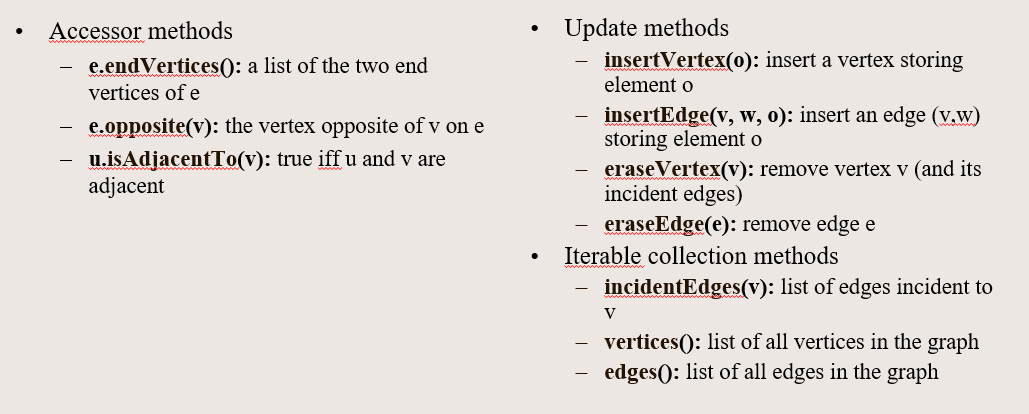
\includegraphics[width=4in]{ds-exam3/graph-adt.png}
\end{center}



\vspace{10pt}
{\bf Question \showmcounter.} 
The {\em square} of a directed graph $G=(V,E)$ is the graph $G^2=(V, E')$ such that
$u,v \in E'$ if and only if $G$ contains a path with at most two edges between $u$ and $v$.
(Namely, $G^2$ contains all the edges of the original graph $G$ plus also new edges 
$(u,v)$ whenever there exists a path $u \rightarrow w \rightarrow v$ for some $w \in G$.)

{\bf (A)} Describe a "brute force" procedure to find the adjacency matrix of $G^2$ 
given the adjacency matrix of $G$. Find its worst-case time complexity as a function 
of $n = |V|$.\\
{\bf (B)} Describe a "brute force" procedure to find the adjacency list representation of $G^2$ 
given the adjacency list representation of $G$. Find its worst-case time complexity.



\item {\bf Given a directed or undirected graph, traverse its vertices in BFS order.}

{\footnotesize BFS traversal is a procedure that adds more information to the vertices and edges of the 
graph. Namely, each vertex changes colors from white (undiscovered) to gray (discovered and inserted 
into the queue of BFS) to black (fully processed with all its neighbors added
to the queue). Each vertex also gets attributes "p" -- its pointer to the parent and 
"d" -- its distance to the BFS root.

\begin{center}
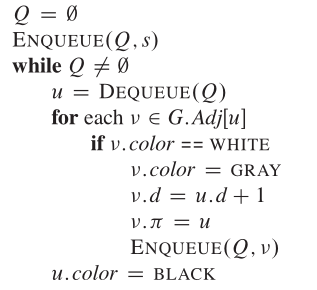
\includegraphics[width=2in]{ds-exam3/bfs-pseudocode.png}
\end{center}
}



\vspace{10pt}
{\bf Question \showmcounter.} 
Assume that the graph $G(V,E)$ is given by an adjacency matrix of size $n \times n$, 
where $n = |V|$ is the number of vertices. The graph also has $m = |E|$ edges.
Assume that we run the BFS traversal to create the BFS tree in the graph $G$. 
Express its time complexity in terms of $n$ and $m$. 

\vspace{10pt}
{\bf Question \showmcounter.} 
The {\em square} of a directed graph $G=(V,E)$ is the graph $G^2=(V, E')$ such that
$u,v \in E'$ if and only if $G$ contains a path with at most two edges between $u$ and $v$.

Assume that somebody runs the BFS traversal two times -- on the original graph $G$
and also on its square $G^2$. During that process 
two BFS trees are obtained -- name them $T$ and $T'$ respectively. 
There are also two queues used during the BFS search -- name them $Q$ and $Q'$ respectively.
Consider the following parameters:

{\bf (A)} $maxlen(Q)$ and $maxlen(Q')$ are the maximum lengths of queues $Q$ and $Q'$ respectively 
during the execution of BFS.\\
{\bf (B)} $maxchildren(T)$ and $maxchildren(T')$ denote the maximum number of children of any node in 
the trees $T$ and $T'$ respectively.\\
{\bf (C)} $height(T)$ and $height(T')$ denote the height of the trees $T$ and $T'$ respectively.

Write the estimates for $maxlen(Q')$, $maxchildren(T')$, $height(T')$, if we know the parameters
$maxlen(Q)$, $maxchildren(T)$, and $height(T)$.





\item {\bf Given a directed or undirected graph, traverse its vertices in DFS order.}
{\footnotesize Traversal algorithms include coloring vertices (as white -- unvisited, gray -- being processed and 
black -- exited), classifying edges (discovery edges, fordward edges, back edges and cross edges)
creating time labels for discovery and finish times.}




\item {\bf Given a graph, find paths or cycles using BFS or DFS traversals.}
{\footnotesize 
Use BFS to find the shortest path from some vertex $v$ to other vertices in the graph.
}
\end{enumerate}












\section{Run and Analyze Graph Algorithms}
\setcounter{mcounter}{0}


\begin{enumerate}[label=2.\Alph*.]
\item {\bf Given a directed graph find its topological sorting or find a cycle.}
Run the algorithm for topological sorting on a graph or estimate its worst-case time complexity
in terms of vertice and edge counts ($n$ and $m$ respectively).

\vspace{10pt}
{\bf Question \showmcounter.} 
Assume that the topological sorting of the vertices in the graph is {\tt U, T, F, P, W, N, E, D}. 
Assume that this order is obtained by reversing the exit times of some DFS traversal. 
Draw the $8$ vertices and show only "discovery edges" belonging to those DFS traversal trees that created this
topological sorting order. You will get one or more DFS trees (specify the order in which these trees are visited). 

\begin{center}
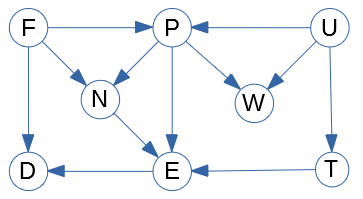
\includegraphics[width=1.4in]{ds-exam3/topological-sort.png}
\end{center}

{\bf Node.} DFS for topological sorting always works, 
since a node in DFS traversal is never exited before a node it points to is exited.


\item {\bf Given a directed graph find its strongly connected components.}

\item {\bf Shortest paths with Dijkstra's or Bellman-Ford algorithm in a graph.} 
Shortest paths are found either by a faster Dijkstra's algorithm (but only positive edges), 
or Bellman-Ford algorithm (both positive and negative edges).

\item {\bf Given a directed acyclic graph, compute its transitive closure.}
Transitive closure (also mentioned in Discrete structures) 
can be done using Floyd-Warshall's algorithm. 
It is also used to find all pairs shortest paths. 

{\bf Theory.} Let $G(V,E)$ be a directed graph (possibly with weights on edges, 
but you can also define all edges with the same weight $1$). 
Define the following $n \times n$ matrix of weights $W = (w_{ij})$: 

\[ w_{ij} = \left\{ \begin{array}{ll}
0, & \mbox{if $i = j$}\\
\mbox{weight of edge $(v_i,v_j)$,} & \mbox{if edge exists}\\
\infty & \mbox{if edge does not exist}\\
\end{array} \right. \]

We can assume that this graph can have negative-weight edges (but it 
must not have negative weight cycles). 
The algorithm to find the shortest paths between 
any two vertices in graph $G$ is the $O(n^3)$ worst-case 
time complexity algorithm given by this pseudocode: 

\begin{center}
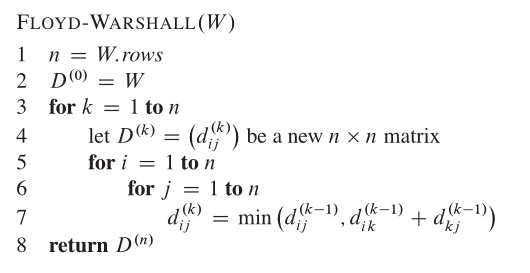
\includegraphics[width=3in]{ds-exam3/floyd-warshall.png}
\end{center}


\vspace{10pt}
{\bf Question \showmcounter.}
Given the directed graph shown in the picture, find the distances 
between any two vertices in this graph -- represent the vertices 
as a $4 \times 4$ matrix $D^{(0)} = (d^{(0)}_{ij}) = (w_{ij})$ where 
the rows and the columns correspond to the vertices $A,B,C,D$ (in this order),
but $d_{ij}$ is initialized to the weights of edges in the graph.


\begin{center}
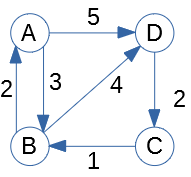
\includegraphics[width=0.8in]{ds-exam3/all-pairs-paths.png}
\end{center}

% https://www.programiz.com/dsa/floyd-warshall-algorithm
Show the matrices $D^{(1)}$, $D^{(2)}$, $D^{(3)}$, $D^{(4)}$
that have elements $d^{(k)}_{ij}$ showing what is the
shortest path from $v_i$ to $v_j$ using either the shortest
path $v_i \leadsto v_j$ found in an earlier iteration or the path 
$v_i \leadsto v_k \leadsto v_j$ going through the vertex $v_k$ (whichever is shorter). 






\item {\bf Given an undirected graph, find its MST using Prim’s or Kruskal’s algorithm.}
Run Prim's and Kruskal's algorithm, analyze its worst-case time complexity 
for different graph representations (adjacency matrices and adjacency lists). 


\vspace{10pt}
{\bf Question \showmcounter.} Consider the following graph $G(V,E)$ with weighted edges. 

\begin{center}
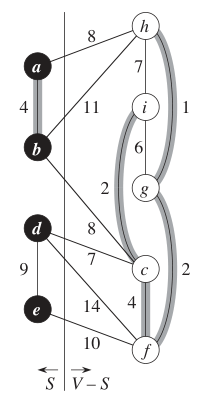
\includegraphics[width=0.8in]{ds-exam3/mst-graph-with-cut.png}
\end{center}

The vertices are split into two disjoint sets $S$ and $V-S$ (separated by a vertical line). 
Such splits of vertices are named {\em cuts} (flows are also used for maximum flow algorithms).
Some edges in this graph are already added to a MST (they are highlighted and shown thicker and darker).

{\bf (A)} Which edge that goes across the cut (connects a vertex from $S$ to a vertex from $V-S$)
is such that it is "safe" to add to the existing MST edges so that we can build a valid Minimum Spanning 
Tree with keeping this edge.\\
{\bf (B)} In how many ways can you add all the missing edges to the existing/highlighted edges 
so that you get a complete MST?


\vspace{10pt}
{\bf Question \showmcounter.} 
Given a graph $G(V,E)$ with $n$ vertices and $m$ edges, the complexity of the Prim's algorithm is 
$O(m \log n)$ (you need to loop over all $m$ edges; and 
one operation of manipulating the priority queue costs $O(\log n)$). 

Describe a variant of Prim's algorithm that runs on the matrix representation of the graph in $O(n^2)$ time. 



\item {\bf Run Ford-Fulkerson or Edmonds-Karp algorithm to find the maximum flow.}
Similar to Assignment 10. 
\end{enumerate}











\section{Use and Analyze Maps, Sets and Hashing}
\setcounter{mcounter}{0}

\begin{enumerate}[label=3.\Alph*.]
\item {\bf Find time complexity for a Map ADT function (hashing, BST, list implementation).} 
We want to implement the Map ADT (typically, a single function therein), 
and we use some underlying data structure -- it may be less efficient than the typical choice (hashing). 
In this task you can write the pseudocode to implement this Map ADT function and estimate 
its time complexity. 


\vspace{10pt}
{\bf Question \showmcounter.}

The Map ADT is shown below: 

\begin{center}
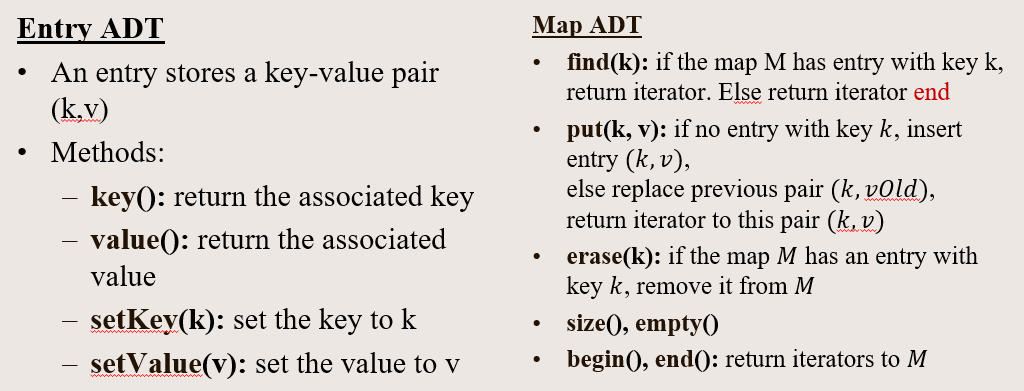
\includegraphics[width=3in]{ds-exam3/map-adt.png}
\end{center}

Describe, how to implement {\tt find(...)}, {\tt put(...)} and {\tt erase(...)}
using the underlying data structure. 

{\bf (A)} Implement map ADT using just some instances of "stack" data structure (instructors know how to implement
{\tt Map[Keys,Values]} with two instances of {\tt Stack[Keys]} and two instances of 
{\tt Stack[Values]}).\\
{\bf (B)} Implement map ADT using a Binary Search Tree (BST).\\
{\bf (C)} Implement map ADT using a hashtable.

For each of the three methods and three functions find the worst-case time complexity 
as $O(f(n))$, where $n$ -- the number of entries in Map right before the function is called.

\item {\bf Given a hash function, identify collisions or estimate probabilities of collisions.} 
The task provides a hash function definition in mathematical notation
(or a prehash function and a module);
we want to compute specific values or estimate the probabilities of collisions.
You may need to use computer simulation to find this. 



\item {\bf Analyze hash table data structures, if collisions are resolved by chaining.}
Given a hashing method, 
\item {\bf Build hash tables, if collisions are resolved by linear probing.}
In this problem hashtable uses open addressing (all the keys and their values are entered
in a linear table). Hash collisions are resolved by probing (and picking the first empty slot). 
For this data structure deletion has to be done carefully (inserting {\tt MISSING} entries
whenever new gaps are created). 
\item {\bf Run and analyze rolling hash – polynomial and cyclic polynomial variants.}

\vspace{10pt}
{\bf Question \showmcounter.}
Consider the following rolling hash function: 

\[ H = s^{k-1}(h( c_1 )) \oplus s^{k-2}( h(c_2) )  \oplus \ldots \oplus  s( h(c_{k-1}) ) \oplus   h(c_k). \]

It is defined for a sequence (sliding window)
of $k$ characters $c_1,\ldots,c_k$, where $s^i(byte)$ denotes left rotating shift of 
$8$ bits. For example $s^3(\mathtt{10001010}) = \mathtt{01010100}$ means shifting all 
bits 3 positions to the left (and append the bits that are "shift out" to the very end). 

{\bf (A)} Find the value of $H("ABC")$, where the hashvalues $h(\ldots)$ of letters "A", "B", "C", etc. 
are their ASCII codes (see \url{https://www.asciitable.com/}).\\
{\bf (B)} Find the value of $H("ABCD")$ as you append one new letter "D". 
Write the expression to compute it using $H("ABC")$ (without scanning the letters "ABC" once again).\\
{\bf (C)} Find the value of $H("BCD")$ as you skip the first letter "A". 

\end{enumerate}


\section{Use and Analyze String Search Algorithms}
\setcounter{mcounter}{0}

\begin{enumerate}[label=4.\Alph*.]
\item {\bf Run and analyze naive string search algorithm.} 
Analyze the speed of naive string search assuming something about the
distribution of input data. 

\vspace{10pt}
{\bf Question \showmcounter.}
Count the number of comparisons in the naive string search algorithm 
as it finds pattern $P = \mathtt{0001}$ in the text $T = \mathtt{000010001010001}$. 
Draw the alignments of pattern $P$ under the text and circle all those characters
that need to be compared for each alignment. 
Then count how many of characters were circled.

\vspace{10pt}
{\bf Question \showmcounter.}
Suppose that pattern $P$ and text $T$ are randomly chosen strings of length $m$ and $n$,
respectively. Both are written in an alphabet $\Sigma$ of size $|\Sigma| = 10$. 
Since $P$ and $T$ are both random, the probability that any two characters will match is
$p =  1/|\Sigma| = 1/10$. Estimate the expected number of character comparisons in the 
naive search algorithm using parameters $m$ and $n$.





\item {\bf Run and analyze Rabin-Karp algorithm with a given rolling hash function.}
%https://brilliant.org/wiki/rabin-karp-algorithm/

\vspace{10pt}
{\bf Question \showmcounter.}
Assume that your alphabet is all $10$ digits; 
the rolling hash function is division modulo $q = 11$. 
Write the formulas for $RH.skip(c)$ and $RH.append(c)$ functions.

\vspace{10pt}
{\bf Question \showmcounter.}
Assume that your alphabet is all $10$ digits; 
the rolling hash function is division modulo $q = 11$. 
You want to find pattern $P = \mathtt{"26"}$ in the text
$T = \mathtt{"3141592653589793"}$. 
How many misleading ({\em spurious}) cache hits happen when 
running Rabin-Karp algorithm?





\item {\bf Run and analyze KMP algorithm, the prefix function used by this algorithm.}

\vspace{10pt}
{\bf Question \showmcounter.}
% https://www.csie.ntu.edu.tw/~hsinmu/courses/_media/dsa_17spring/dsa_2017_hw2_sol_1.pdf
In the string $T = \mathtt{947892879497}$ find the pattern $P = \mathtt{9497}$.

{\bf (A)} Find the prefix function $\pi(i)$ used by the Knuth-Morris-Pratt algorithm.\\
{\bf (B)} Draw all the alignments of pattern $P$ under the text $T$ that are checked
by the Knuth-Morris-Pratt algorithm and circle the characters that are being compared. 
Count the total number of compared characters.


\item {\bf Run NFA on a string, describe languages accepted.}
Similar to the Assignment 14.

\item {\bf Convert NFAs to regular expressions and vice versa.}
Similar to the Assignment 14.



\item {\bf Write regular expressions to match, search or substitute certain string patterns.}

\vspace{10pt}
{\bf Question \showmcounter.}
Postal codes in Canada (see \url{https://bit.ly/3dlyVU4}) follow the convention 
that they consist of 6 symbols -- alternating sequence of uppercase Latin letters and digits. 
Use the function {\tt re.sub(...)} as in Python to swap two parts of a postal code. 
For example, the code {\tt K1A0B1} should become {\tt 0B1K1A}.
Your regular expression should work on a single string (one line of text) 
and swap only those postal codes which are enclosed by 
word boundaries (for example, words {\tt xxxK1A0B1} or {\tt K1A0B1yyy} should not 
be recognized as postal codes and no swapping should occur.
\begin{center}
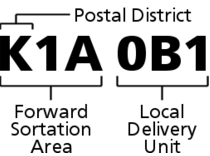
\includegraphics[width=1.5in]{ds-exam3/canadian-postal-code.png}
\end{center}

\vspace{10pt}
{\bf Question \showmcounter.}
Write a regular expression to recognize all those strings that contain only digits
and represent integer numbers divisible by 8. Use the Python function {\tt re.fullmatch(...)}.

\vspace{10pt}
{\bf Question \showmcounter.}
Write a regular expression to find all 8-digit sequences and prepend 
the Latvia area code. For example, a phone number {\tt 12345678} should become
{\tt +371-12345678}. 




\item {\bf Build a "trie" from the given set of strings.}
A trie shows common prefixes; it can be used to find the 
predecessor for the given pattern $P$ in time linear in $|P|$.

\vspace{10pt}
{\bf Question \showmcounter.}
Consider the following strings:
%ALARM$, ALAS$, ALL$, ALLEY$, ALLOW$, ALLOY$, ALLY$
%ARE$, AREA$, ARENA$, ARM$, ARMED$, ARMS$, ARMY$
\begin{verbatim}
BAR$, BARE$, BEAR$, BEARD$, BEARER$, BEER$, BEE$, BIRD$
\end{verbatim}
{\bf (A)} Draw a {\em trie} for the following collection of $8$ strings. 
The strings are written in an alphabet containing all $26$ uppercase 
letters, and dollar sign alphabetically precedes all of them (and the 
separating commas and spaces are not part of the alphabet).\\
{\bf (B)} How many edges can be compressed in this trie?\\
{\bf (C)} Write a word that is not among the $8$ strings and would need the most string comparisons 
before we locate its predecessor in the trie.

\vspace{10pt}
{\bf Question \showmcounter.}
Assume that the alphabet $\Sigma$ being used to store a trie with $n$ 
nodes has a large number of letters $d = |\Sigma|$ (such as Unicode with up to $65536$ 
symbols or something like that). 
A single node in the trie can be implemented in various ways -- for each method 
estimate the space taken by this tree and also the worst-case time to search for a pattern $P$
containing $|P| = m$ characters. 

{\bf (A)} Every node of a trie is itself implemented as a binary 
search tree with the letters from $\Sigma$ being used as the search keys.\\
{\bf (B)} Every node of a trie is implemented as a linked list 
with letters from $\Sigma$ linked in nodes with additional pointers going to the child nodes.\\
{\bf (C)} Every node of a trie is implemented as a hash table with 
letters from $\Sigma$ being used as hash keys.





\item {\bf Convert "trie" to an LCP array; convert an array to a Cartesian tree.}

\vspace{10pt}
{\bf Question \showmcounter.}
Consider the following strings: 
\begin{verbatim}
ALARM$, ALAS$, ALL$, ALLEGE$, $ALLELE, ALLEY$, ALLOW$, ALLOY$, ALLY$
\end{verbatim}

{\bf (A)} Build an array showing the longest common prefix (LCP) information for any two alphabetically adjacent
strings from this list.\\
{\bf (B)} Create a Cartesian tree from the array built in the previous step.\\
{\bf (C)} Show the longest common prefix of two strings: {\tt ALARM} and {\tt ALLEY} 
in both the LCP array and the related Cartesian tree. 


\item {\bf Build a suffix tree/array, show how it can answer a given search query.}
A suffix tree is a trie built from suffixes taken from one or more strings
(and suffix array is the longest common prefix information for that trie). 
They can be used to answer the least common ancestor (LCA) and range-minimum queries (RMQ).


\vspace{10pt}
{\bf Question \showmcounter.}
The image below shows a suffix tree that is built from the following two strings:
$P = \textcolor{blue}{\mathtt{BANANA\$}}$, 
$P_{rev} = \textcolor{green}{\mathtt{ANANAB\#}}$.\\
$P_{rev}$ is string $P$ reversed. Two different end-markers are used:
$\texttt{\$}$ (original string) and $\texttt{\#}$ (reversed string). 

\begin{center}
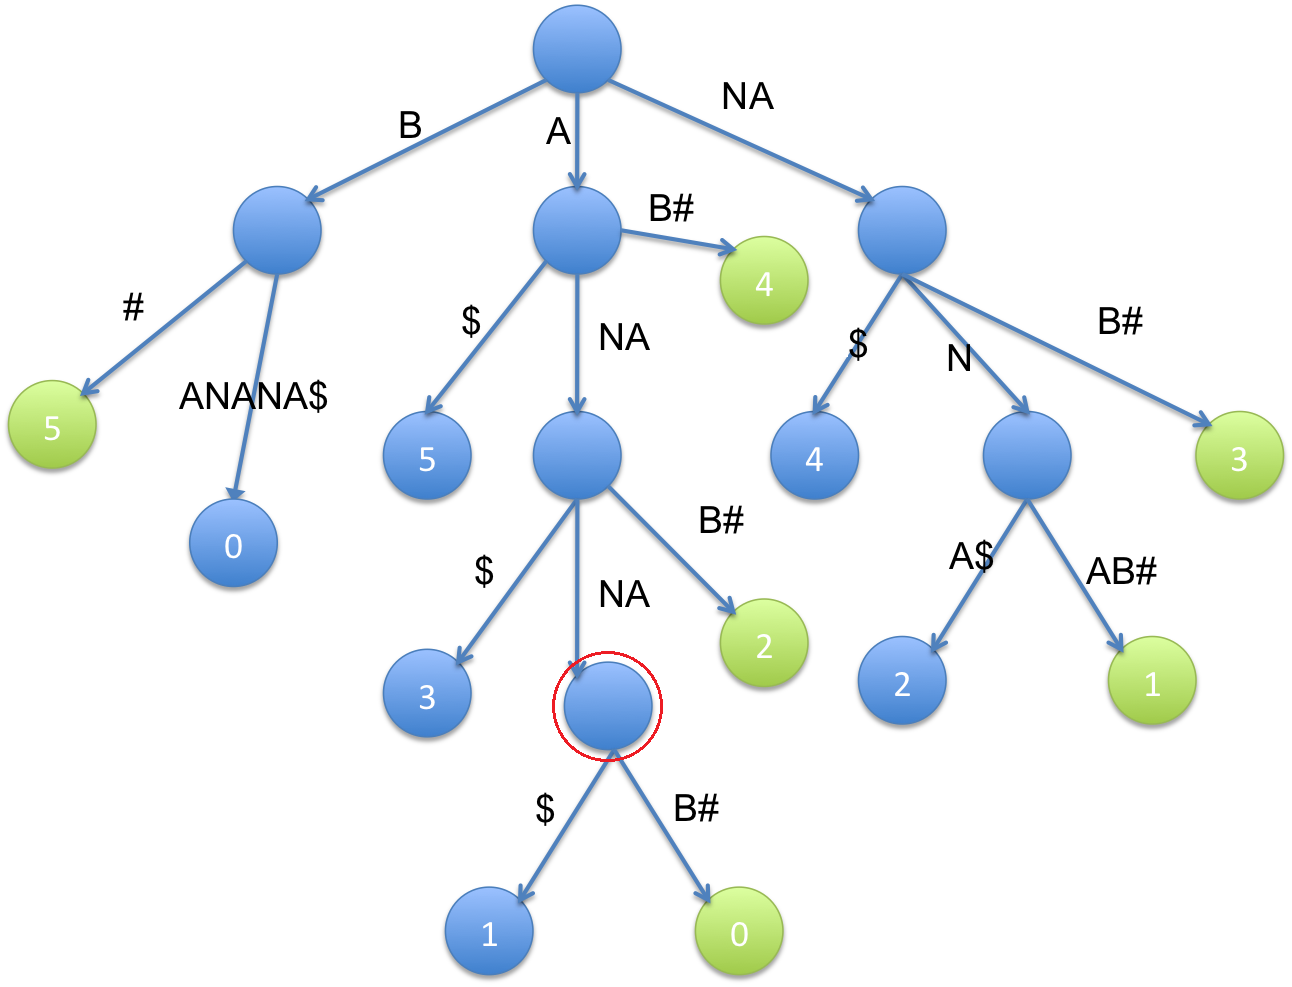
\includegraphics[width=2.6in]{ds-exam3/banana-suffix-tree.png}
\end{center}

All the leaves that are suffixes of the original string are shown in blue, but all 
the leaves that are suffixes of the reversed string are shown in green. 
The tree contains a circled vertex with the following property: It is the deepest inner 
node that has both blue and green successors.
It also turns out that {\tt ANANA} the longest palindrome 
that belongs to both $P$ and $P_{rev}$. 

{\bf (A)} If we replace $P = \mathtt{BANANA}$ with an arbitrary string in this example, 
will the deepest inner node with both blue and green successors be a substring to both 
$P$ and $P_{rev}$?\\
{\bf (B)} Will the deepest node be a palindrome? Can this suffix tree find the longest
palindrome contained in $P$.\\
{\bf (C)} Describe the brute-force algorithm finding the longest palindrome contained within 
the pattern $P$. What is its time complexity?

\end{enumerate}


\clearpage

{\LARGE Answers}

{\bf Topics 1A--1E: Use graph representations and graph properties.} 

\begin{enumerate}
\item $2m = deg(v_1) + \ldots + deg(v_n)$. The largest value for $2m$ is $5n$, the smallest value is $3n$. 
Once we express $n$ from these inequalities, we get $2m/5 \leq n \leq 2m/3$. 
\item The largest number of edges is $45$ (full graph of $10$ vertices plus two more isolated vertices). 
\item Observe that all in-degrees and out-degrees should equal $5$ (otherwise the in-arrow count would 
differ from the out-arrow count). The number of nodes $n \geq 6$; if you know the number of edges $m$, 
then $n = m/5$. 
\item For example, consider the adjacency matrix and two ADT functions.
In order to find {\tt e.endVertices()} for the given edge $(v_i, v_j)$ 
just look at the column and row index (it is $O(1)$ time). 
For {\tt insertVertex(o)} you need to allocate a larger matrix, 
so it is $O(n^2)$ time.
\item {\bf (A)} Procedure is similar to matrix multiplication; 
it normally takes $O(n^3)$ steps (you can also speed up using 
Strassen's algorithm). {\bf (B)} For each vertex 
you need to scan all the edges in the adjacency lists, 
it takes $O(n \cdot m)$. 
\item It is typically more efficient to run BFS on adjacency lists. 
If you must use adjacency matrix, then you need to visit all edges
and for each edge scan one line of the matrix. 
It takes $O(n \cdot m)$. 
\item {\bf (A)} Graph $G^2$ is more dense, the "breadth" 
of each level in the original tree grows by a factor 
$maxdegree(v)$  (maximum degree in the original graph $G$). 
\end{enumerate}



{\bf Topics 2A--2F: Run and Analyze Graph Algorithms.} 

TBD


{\bf Topics 3A--3E: Use and Analyze Maps, Sets and Hashing}

TBD


{\bf Topics 4A--4I: Use and Analyze String Search Algorithms.}

TBD

%\begin{enumerate}
%\item The trie is shown in the image below:
%\begin{center}
%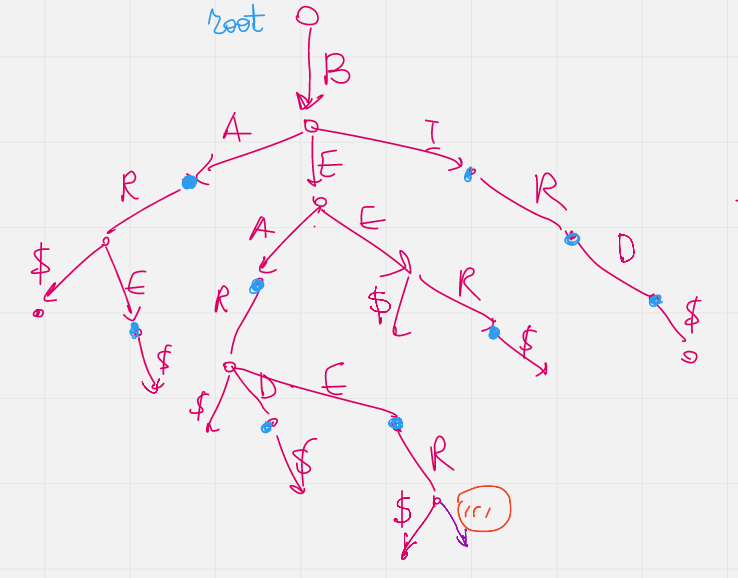
\includegraphics[width=2in]{ds-exam3/search-trie.png}
%\end{center}
%\item {\bf (A)} Yes.\\
%{\bf (B)} Not necessarily - e.g.\ {\tt "ABAB"} and {\tt "BABA"} may 
%both be contained in $P$, but they are not palindromes; and {\tt "ABABA"} or {\tt "BABAB"} may %both be absent from $P$.
%(Suffix trees can find palindromes, but the construction is not that straightforward.)\\
%{\bf (C)} Can try all $O(n^2)$ substrings, and check which ones are palindromes in $O(n)$ %time; total time $O(n^3)$. 
%\end{enumerate}


\end{document}
